\chapter{Implementation}
This chapter discusses the implementation of adaptive learning and pitch detection techniques in the form of a web application. I use a variety of software libraries and frameworks to facilitate this, and these are mentioned, as well as a justification of my platform choice. The use implementation of a segmented autocorrelation algorithm to handle pitch detection is discussed, as well as key error correction ideas. Further to this, we discuss the server's handling of user data and its adaptive algorithms.
	\begin{figure}[h]
	\centering
	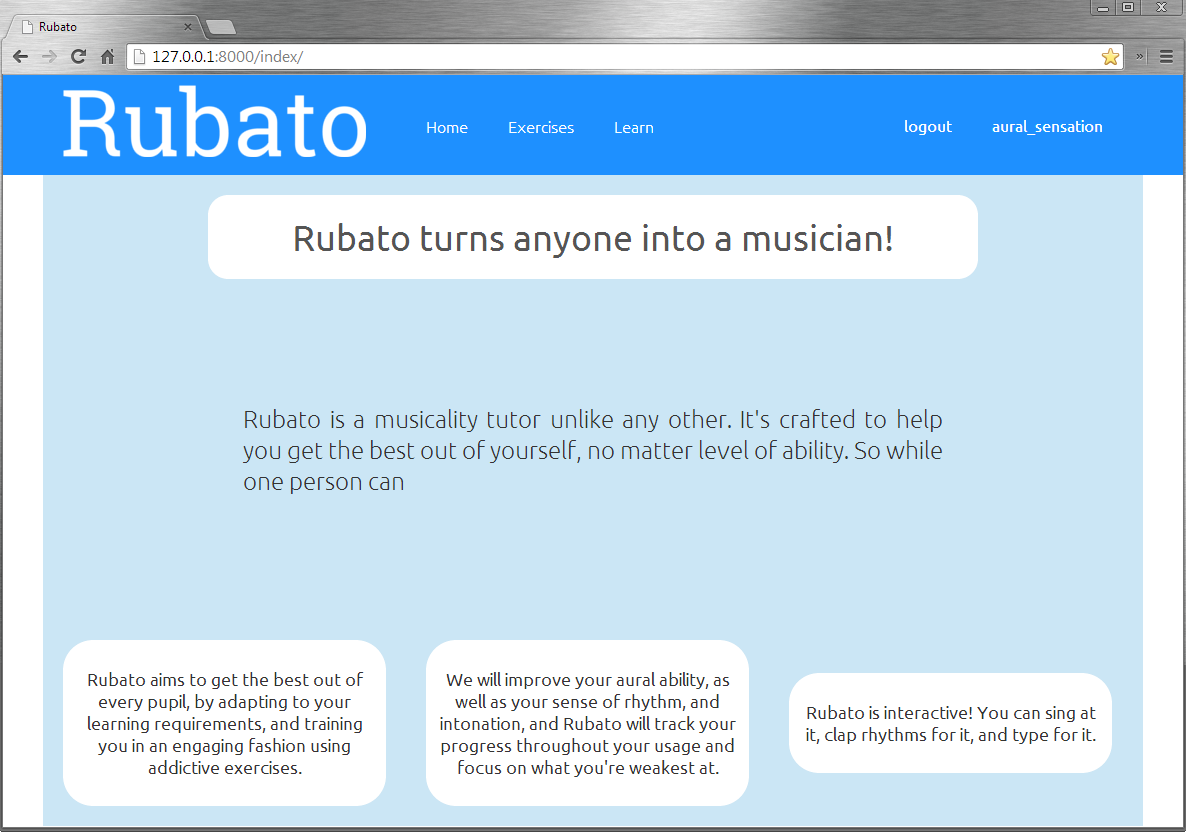
\includegraphics[scale=0.4]{webpage.png}
	\caption{The home page of the website}
\end{figure}
	\section{Platform choice}
	As the modern internet browser has become more and more powerful, web apps have been able to reduce the previous speed disadvantages they faced when compared with their native equivalents. The web-platform is advantageous due to having a singular codebase, meaning that it can be used by anyone with a web browser, independent of their device, so it has the potential to reach more users. Another key advantage of building a web app is that as user testing is so key to evaluating the app's success, when the time comes, and I want to show it to users, I can easily point people to my website and people will know how to get to it. Distributing a mobile app to others for testing purposes is painful, and difficult to update once they have installed it, with a web app I can instantly change the build of my website, and whoever is testing it won't have to do anything more than refresh the page to get the latest changes.
	\subsection{Mobile browsing}
	While the application is not available is a native Android or iOS application, on Android, it can be run in browser as Google Chrome supports the Web Audio API. Unfortunately, support of this library is limited on iOS, and it can only support audio playback, and not audio capture from a microphone source.
	
	\section{Application stack}
	\begin{figure}[h]
		\centering
		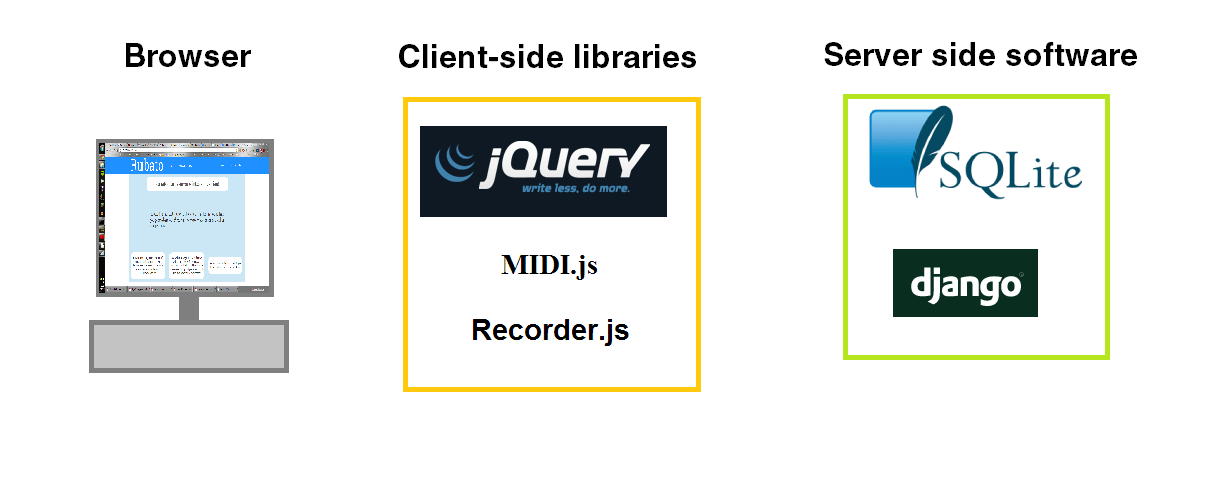
\includegraphics[scale=0.4]{application_stack.png}
		\caption{The 2-tier application stack for Rubato, showing client and server side technologies used}
	\end{figure}
	\section{Server-side software}
	\subsection{Django web framework}
	The Django web framework\cite{django} allows web developers to create complex web applications quickly, and with little fuss. It is based on the Python language which is known for its emphasis on readability and speed of development.
	It also includes a simple web server for development purposes, and this is what we have used throughout the project. If this application was ever deployed widely, then we would need to consider using a proper web server like Apache or Nginx, both of which have django bindings, because the Django development server does not have the necessary security checks to ensure it is not prone to malicious attacks. This doesn't really affect the behaviour of the web app, so using the development server makes more sense, as it easy to configure, run, and restart.
	\subsection{SQLite}
	SQLite is a self contained, serverless database that comes preconfigured to use with Django. Django Models (discussed later in this chapter) essentially deal with all database activity for us, so it is unimportant to know what goes on inside the SQLite database.
	\section{Client side JavaScript libraries}
	We use multiple Javascript libraries to deal with common tasks like recording audio, audio playback, and asynchronous communication with the server.
	
	\subsection{Recorder.js and the Web Audio API}
	Recorder.js and the Web Audio API allow us to seamlessly capture audio in the browser. To start with, we must create an AudioContext.
	\begin{lstlisting}
	var mediaStreamSource = new webkitAudioContext();
	\end{lstlisting}
	If we want to any sort of audio work in the browser, this is the object that the Web Audio API requires us to use. It represents a series of audio modules linked together that form some sort of audio processing pathway.
	 For the purpose of capturing audio from the microphone, we need to create a MediaStreamSourceNode() within the context.
	\begin{lstlisting}
	var mediaStreamSource = context.createMediaStreamSource(s);
	\end{lstlisting}
	Once we've done this, Recorder.js comes into play. It is simply a matter of running  the following command
	\begin{lstlisting}	
	recorder = new Recorder(mediaStreamSource);
    recorder.record();
	\end{lstlisting}
	and we can start recording media. When we want to stop we can use 
	\begin{lstlisting}	
	recorder.stop();
	\end{lstlisting}
	
	\subsection{MIDI.js}
	 MIDI.js provides us with a way to synthesise audio playback in browser. Once we've set up the plugin, we simply have to call the following function to play a note of our choosing
	 \begin{lstlisting}	 
		function playNote(){
		    var delay = 0; // play one note every quarter second
		    var note = MIDI_note; // the note's pitch in MIDI notation
		    var velocity = 127; // how hard the note hits
		    // play the note
		    MIDI.setVolume(0, 127);
		    MIDI.noteOn(0, note, velocity, delay);
		    MIDI.noteOff(0, note, delay + 0.75);
		}
	\end{lstlisting}
	
	\subsection{JQuery}
	The JQuery library enhances the functionality of vanilla HTML and JavaScript by providing various utility methods/simplifying existing methods. We use it to dynamically update elements on the page, and importantly, to communicate with Django via AJAX (Asynchronous JavaScript and XML). The idea of AJAX is to be able to communicate to the server without reloading the page, and we will use it to facilitate adaptive learning, which will be discussed further in Section 3.11.
	
\section{Pitch Detection}
\par Pitch detection is an important part of the exercises, and as such, robust pitch detection has been an important feature in the development of this program. 
\par Most existing pitch detection algorithms are based on real-time applications, i.e. where audio captured from a microphone is analysed and the pitch is displayed as a constantly updating function of the audio signal. This is useful for applications like guitar tuning, where you need near instant feedback, and you can be sure that the pitch you are inputting is fairly constant. 
\par With analysis of pitch in the human voice however, the problem is that even with well trained singers, the pitch of a note can vary quite considerable over a 2 second period, due to vibrato\footnote{Vibrato is the musical technique of intentionally oscillating the pitch of the note around a fixed point.}, or other causes that can be hard to pick up just by listening to yourself, so it is not always trivial to determine one pitch to summarise a sample of a single held note, and indeed, often not appropriate to do so if the singer cannot even stay on the same note for that short period of time, and wobbles around the note inconsistently.
\par It is with this in mind that I have developed a Segmented Autocorrelation Algorithm,  that can accurately determine the pitch of a 2-3 second sample of singing.

\subsection{Segmented Autocorrelation Algorithm}
The principle of the Segmented Autocorrelation Algorithm is relatively simple: A given audio sample is split into several segments, pitch detection is run on each segment, and then the segments are analysed to calculate pitch. I have also employed several error detection/correction methods that are detailed below.
\begin{figure}
	\centering
	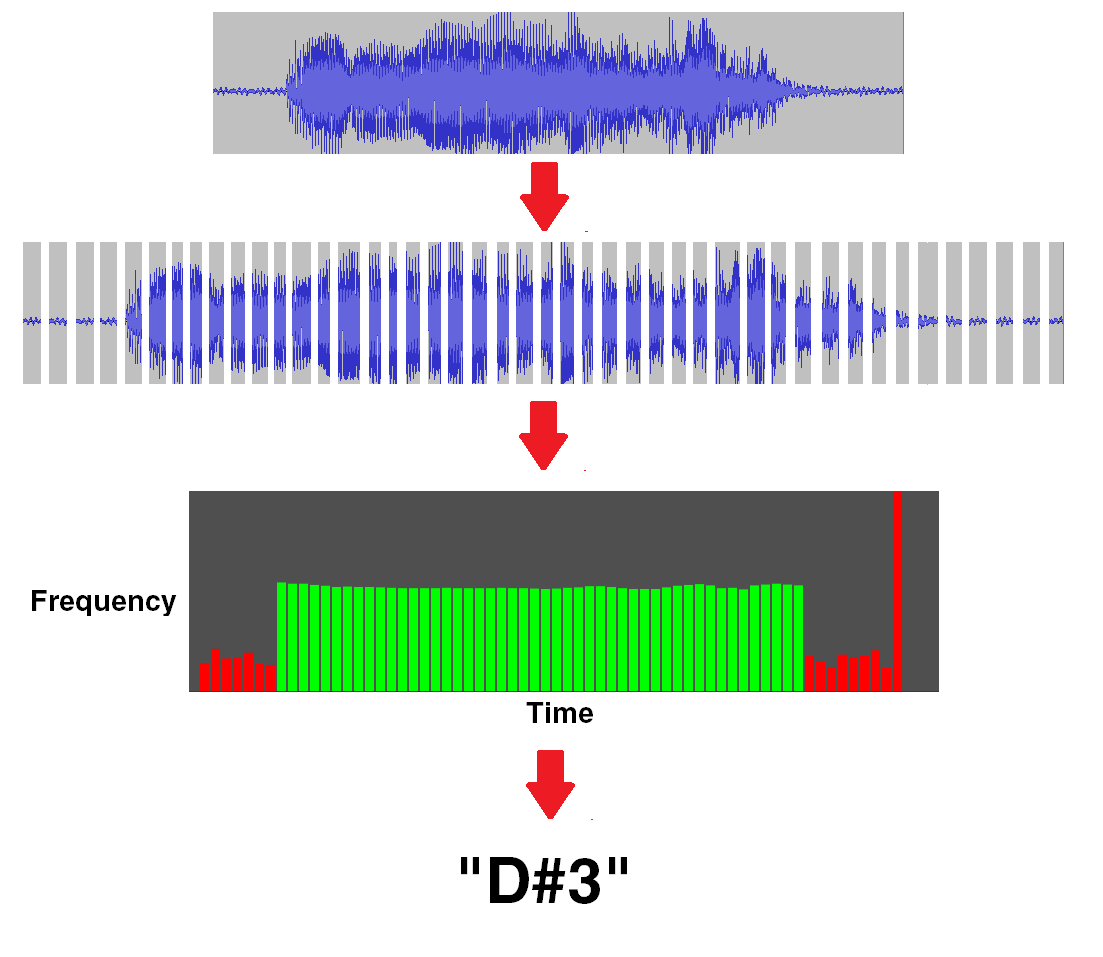
\includegraphics[scale=0.5]{segmented_autocorrelation.png}
	\caption{An illustration Segmented Autocorrelation. In the first image, we have the original source audio stored in uncompressed PCM format, with time on the \(x\) and amplitude on the \(y\), in the next image it is broken into several equally sized segments of length 1200 samples, and then each of these segments is analysed using autocorrelation to give a frequency reading, shown on the third panel. Red portions represent data discarded as junk by the algorithm}. These are then analysed to give a final pitch reading for the given audio sample.
\end{figure}

\subsection{Breaking it apart}
The first step in the algorithm is to segment the audio signal, this allows us to individually analyse the pitch of each segment, so that if the pitch varies, we can detect it.
\subsubsection{Choosing a segment size}
\par Most PC microphones sample audio at either 44,100Hz or 48,000Hz, as these ensure that the full 20KHz spectrum of human hearing can be recorded due to the Nyquist–Shannon sampling theorem (see Background Section 2.5). For the sake of simplicity we will assume a sample rate of 48,000Hz for this report, though the program can handle either rate.
\par The human vocal range defined in Section 2.4.2 was E2 - C6, which corresponds to a frequency range of ~80-1000hz\cite{scientificPitchTable}. To calculate the number of samples at either end of the range: 
 		 \[48000\div 96 = 600 \text{ samples}\] 
		 \[48000\div 1000 = 48 \text{ samples}\]
		
\par In order for our autocorrelation algorithm to work, it is  necessary to take a segment size at least twice that of the lowest frequency we wish to sample.
This is because in autocorrelation, we must compare the signal with an offset version of itself, and this score is maximal with an offset equal to the period of the signal. Therefore, in our example, if we use anything less than a 1200 sample size and are trying to detect a 96Hz signal, we won't even be able to autocorrelate on a full period.  I have therefore decided to use 1200 as the segment size. Increasing this number results in a higher quality analysis per segment, but the trade-off is that segments per second decreases, meaning you are sacrificing granularity of change of pitch over time.

\subsubsection{Autocorrelation}
The algorithm for the pitch analysis for individual segments is the autocorrelation algorithm outlined in the first chapter. It is fast, simple to implement, and we don't mind so much about errors due to the fact that it's not a real-time implementation. This means we can look at each segment in the context of the whole recording, and run error correction algorithms outlined below if we do encounter any dodgy pitch readings.

\begin{lstlisting}
function autoCorrelate(buf, sampleRate){

    var MIN_SAMPLES = 48;	// corresponds to ~1000 Hz  i.e. C6
    var MAX_SAMPLES = 600; // corresponds to ~80hz i.e. E2
    var SIZE = segment_size; //1200
    var best_offset = 0;
    var best_correlation = 0;
    ACF = new Array(MAX_SAMPLES-MIN_SAMPLES+1).
    for (var offset = MIN_SAMPLES; offset <= MAX_SAMPLES; offset++) {
        var correlation = 0;
        var max = SIZE-offset;

        for (var n=0; n<max; n++) {
            correlation += (buf[n])*(buf[n+offset]);
        }

        ACF[offset-MIN_SAMPLES] = correlation

        if (correlation > best_correlation) {
            best_correlation = correlation;
            best_offset = offset;
        }
    }
    
    return sampleRate/best_offset
    
\end{lstlisting}

\subsubsection{Enhancing the results: Quadratic Interpolation}
With autocorrelation, one inherent limitation is the granularity of the detected pitch.
Let's say a we are trying to identify a sung D4. This has a frequency of 293.66Hz and will therefore correspond to a lag of \(48,000Hz/293.66Hz = 163.45 \text{samples}\). Our algorithm at present does not have a way of dealing with fractions of a sample, so at best we will detect 163 or 164 samples. This lack of precision in this case will cause an error of roughly \(\pm 5 \text{cents}\), which isn't too bad. The problem however becomes more significant as we detect notes with higher frequencies, as these notes will correspond to smaller lag times, and thus a discrepancy in lag detected will correspond to a more noticeable error in pitch detection.

\begin{figure}
	\centering
	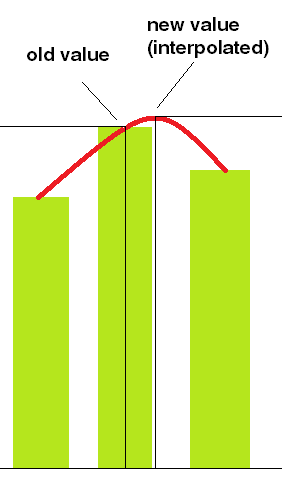
\includegraphics[scale=0.4]{quadratic_interpolation.png}
	\caption{If we simply use the peak of our autocorrelation function to determine the pitch, we limit ourselves to detecting pitches only of discrete intervals. Using quadratic interpolation, we can get a better estimate of the best autocorrelation value}
\end{figure}

One way to solve this problem is quadratic interpolation\cite{quadraticInterpolation}. The idea is to take three points and built a guadratic curve between them. By looking at the maximum of this curve, we can interpolate and find a new peak that will be more accurate.

The equation to calculate the quadratic interpolation for three different point \(x_1<x_2<x_3\) is as follows:

\[x_\text{max} =\frac{1}{2} \frac{B_{23}f(x_1) + B_{31}f(x_2)+ B_{12}f(x_3)}
{d_{23}f(x_1) + d_{31}f(x_2) + d_{12}f(x_3} \]

where:
\[B_{ij} = i^2 - j^2\]
\[d_{ij} = i - j\]

we then simply take our \(x_\text{max}\) and make that into our new offset.  


\subsection{Detecting errors}
There are two primary methods of detecting errors after autocorrelation has been performed.
Firstly, we detemine the active area of the recording, this being the section of the recording where the user is actually singing. To do this, we apply a filtering method based on the RMS Amplitude of the sample.
Secondly, we apply a median filter to the sample to smooth out any clearly anomalous pitch readings detected during the active area.
\subsubsection{Median Filtering}
Median filtering is a noise reduction process used when sharp spikes occur in a signal. It works using a sliding window algorithm, applying a median filter to all the elements in a grid. The code below describes an implementation in Javascript, and Figure 3.2 gives a visualisation of how it works. 
For this application, the median filter is more appropriate than the more standard moving average filter, as it is non-linear meaning that large spikes will be completely removed, not just smoothed over. 
\begin{lstlisting}
function medianFilter(signal,window_size){
    var medians = new Array(signal.length);
    for (var i = mid; i<signal.length-mid; i++){
        var mid = Math.floor(window_size/2);
        var startIndex = i - mid;
        var median_window = new Array(windown_size);
        for (var j = 0; j <window_size; j++){
            median_window[j] = signal[startIndex + j];
            }
        }
        medians[i] = median(median_window);
    }
    return medians;
}
\end{lstlisting}

In my implementation I use window size 3, as large spikes of this sort are fairly rare, and when they do occur they're usually only 1 segment wide.

\begin{figure}
	\centering
    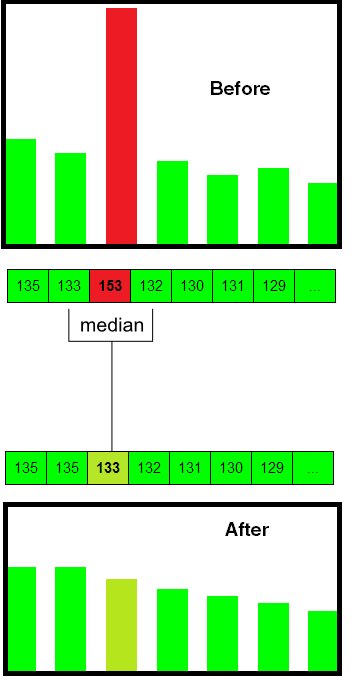
\includegraphics[scale=0.7]{median_demonstration_tall.png}
	\caption{A visualisation of the median filter with window size 3: Each point is transformed to the median of a sample size 3 centered on the point. The red column of height 153 is therefore transformed to median(133,152,132) = 133}
\end{figure}


\subsubsection{Amplitude filtering}
A typical audio sample will have junk data at either end of the recording as the user prepares to sing after activating the microphone, and then leaves the microphone running for a fraction of a second after singing. Amplitude filtering is designed to detect where the edges of the useful data are, and cut them off.

During the autocorrelation, as well as calculating the pitch for each segment, we also calculate its amplitude using root mean square (RMS). It is preferable to use RMS to the conventional peak amplitude method normally used on audio signals, as our window size is sufficiently high that a spike in a given segment due to external noise could cause the amplitude value to be too high. RMS should avoid this as it takes an average over a given sample. The RMS amplitude is calculated using the following algorithm:
 \[\sqrt{\sum_{i=1}^{n} s_i^2/n}\] where \(n\) is the number of samples in the segment, and \(s_i\) is the i-th sample in the segment. After analysing all segments we end up with a result similar to that shown in Figure 3.3, with a block of loudness surrounded by two blocks of quietness.
 
\begin{figure}
	\centering
    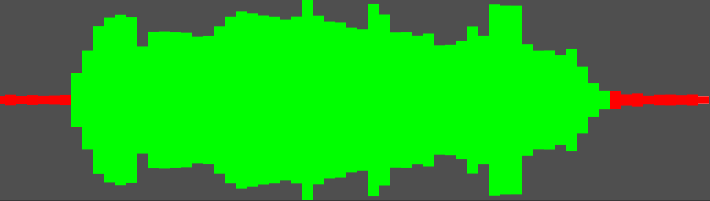
\includegraphics[scale=0.7]{amplitude_filtering.png}
	\caption{A recording of a sung note showing amplitude vs time. The red areas have been filtered our with amplitude filtering}
\end{figure}


\subparagraph{Microphone calibration}
To make sense of this, we have to work out what data should be accepted, and what should be rejected as too quiet to contain valid pitch data. This is done through calibration: The first time the user opens an exercise that uses microphone data, the program records a 2 second sample and segments it similarly to the preprocessing of the autocorrelation method. The minimum amplitude of all segments is then taken as the calibration value, \(a_0\).
When determining which segments to cut off in the amplitude filtering stage, we discard all segments with \(\text{amplitude} < 2a_0\). This value has been determined empirically to be a reasonable threshold for minimum amplitude

\section{Putting it together}
Now that we've determined a suitable chunk of frequencies that represent the pitch of note, we need to work out how to combine them into one reading.
\subsubsection{Rolling standard deviation}
In order to ensure that large contiguous regions of mispredicted pitch that cannot be fixed with median filtering do not throw of our pitch detection , we need to separate the frequencies into regions of fairly close pitch. We do by grouping frequencies into contiguous regions with a standard deviation below a certain threshold. 

Once we have done this, we look for the largest contiguous region in our sample, and calculate pitch by taking the average frequency in the region. If the largest contiguous region is smaller than 60\% of the size of all our valid frequency data, we throw an error, and ask the user to try again as we cannot choose an authoritative region.

\section{Measuring user ability}

User ability is measured through a level system. Every user has a level value assigned to each exercise they attempt, and an overall level also. Users with a high level will not have to start from the beginning when attempting new exercises. 
All users start at at level 1 when they sign up.
To increase their level, the user has to complete exercises correctly. As their level increases, the exercises adapt and get harder.
Measuring user ability is achieved by assigning a score to every \bsq{attempt} at a certain exercise. These scores are then processed by the server to determine:
	\begin{itemize}
		\item Whether the user should be levelled up.
		\item What questions it is best to ask them next.
	\end{itemize}

\subsection{Intonation training}

The scoring system for intonation training is as follows:

\[\text{difference} = |P_\text{actual}- P_\text{target}|\]
\[\text{perfect\_score} = 0.1 \]
\[\text{distance\_from\_perfect} = \text{max}(\text{difference}-\text{perfect\_score},0)\]
\[\text{score} = \text{max}(1 - \text{distance\_from\_perfect},0)\]

Intuitively, this means that any interval attempt less than 0.1 semitones from the actual pitch is classed as a perfect score, and anything over 1.1 semitones away is classed as a zero,with values between those 0.1 and 1.1 semitones determined by linear interpolation.

Every time the user completes an attempt at an interval, their score is calculated and sent to the server. In order to ensure that the exercise is not interrupted, we use Asynchronous Javascript and XML (AJAX) which allows the user to continue playing while their score is communicated to the server in the background. The JQuery library contains support AJAX, and we use it like this.

\begin{lstlisting}
function sendScore(){
    var score = calculateScore();
    var i = interval;
    $.post('/interval/send_score', {score: score.toString(), interval: i.toString()}, function(data){
     });
}
\end{lstlisting}

This simple piece of code sends the score to the server, as well as the interval the score was calculated for.

\section{Adapting to user ability}

When the server recieves the score, we store it in a database, so that we can retain a history of all their past attempts.
Django interfaces with the database through Models. An example of this is the IntervalScore model below. This particular model stores all the information about a user's attempt at singing an interval in the interval training exercise.
		
		\begin{lstlisting}
		class IntervalScore(models.Model):
   			interval = models.ForeignKey(Interval) 
    		timestamp = models.DateTimeField(auto_now_add=True)
    		score = models.FloatField();
		    user = models.PositiveIntegerField();
		    def __str__(self):
        		return " Score: " + str(self.score) + " for" + self.interval.name + " with user id: " + str(self.user)

		\end{lstlisting}
		The interval field represents the interval that the user has attempted, the timestamp tells us when it was attempted, and the score field tells us the calculated score for that attempt.
		
To ensure that the user is tested with an interval appropriate for their skill level, every time the user requires a new interval to attempt, they must request it from the server. The server then obtains their interval score history by querying the database with the User's ID. 

Depending on the level of the user, as well as their history, a different interval will be sent.
\begin{itemize}
	\item If the user's last 3 attempts at a given interval have all been below a certain threshold (calculated using the level of the user), the user will be sent that interval, as well as a prompt to playback the interval and listen to what it sounds like before attempting it agin.
	\item Different intervals are classified into levels, and you can only unlock some of the harder musical intervals (e.g. a major 7th, diminished 5th) once you reach a certain level
	\item Your level is incremented by 0.025 for every musical interval you get correct, and decremented by 0.01 for interval gotten wrong.
\end{itemize}